%%%%%%%%%%%%%%%%%%%%%%%%%%%%%%%%%%%%%%%%%%%%%%%%%%%%%%%%%%%%%%%%%%%%%%%%%%%%%%%%
%2345678901234567890123456789012345678901234567890123456789012345678901234567890
%        1         2         3         4         5         6         7         8

\documentclass[letterpaper, 10 pt, conference]{ieeeconf}  % Comment this line out
                                                          % if you need a4paper
%\documentclass[a4paper, 10pt, conference]{ieeeconf}      % Use this line for a4
                                                          % paper

\IEEEoverridecommandlockouts                              % This command is only
                                                          % needed if you want to
                                                          % use the \thanks command
\overrideIEEEmargins
% See the \addtolength command later in the file to balance the column lengths
% on the last page of the document



% The following packages can be found on http:\\www.ctan.org
\usepackage{graphics} % for pdf, bitmapped graphics files
\usepackage{epsfig} % for postscript graphics files
\usepackage{mathptmx} % assumes new font selection scheme installed
\usepackage{times} % assumes new font selection scheme installed
\usepackage{amsmath} % assumes amsmath package installed
\usepackage{amssymb}  % assumes amsmath package installed
%\usepackage{amsmath,amssymb,amsthm}
%\usepackage{amsthm}
\usepackage[utf8]{inputenc}
%\usepackage{enumitem}
\usepackage{graphicx}
\usepackage[table,xcdraw]{xcolor}
%\usepackage[center]{caption}
\usepackage{scrextend}
\usepackage{comment}
\usepackage{xfrac}

\title{\LARGE \bf
Co-optimization of Application and Architecture
for a Coarse Grained Re-configurable Architecture
}

\author{Christopher Ohara (1322884) \\
Erik Wouters (1325892)
}

\begin{document}

\maketitle
\thispagestyle{empty}
\pagestyle{empty}

%%%%%%%%%%%%%%%%%%%%%%%%%%%%%%%%%%%%%%%%%%%%%%%%%%%%%%%%%%%%%%%%%%%%%%%%%%%%%%%%
\begin{abstract}

This electronic document is a ÒliveÓ template. The various components of your paper [title, text, heads, etc.] are already defined on the style sheet, as illustrated by the portions given in this document.

\end{abstract}

%%%%%%%%%%%%%%%%%%%%%%%%%%%%%%%%%%%%%%%%%%%%%%%%%%%%%%%%%%%%%%%%%%%%%%%%%%%%%%%%
\section{Introduction}

The goal of this report is to describe the process of improving a naive implementation of the Butterworth filter\cite{Podder} that runs on the Course Grain Re-configurable Architecture (\texttt{CGRA}). \texttt{CGRA} provides several types of functional units (\texttt{FU}) that can be wired together by usage of an \texttt{architecture.xml} file, where the components, ports and connections are defined. It supports configuring the connections at run-time by usage of a network description, but such configurations have not been explored in this report, as the benefits would be marginal for this filter.

The \texttt{FUs} run instructions in parallel. Each \texttt{FU} has it's own set of instructions. Their instructions are programmed in Parallel Assembly (\texttt{PASM}). Improvements over the naive implementation are compared by their energy, delay and area and the combined measure of these (\texttt{EDAP}).

The \texttt{CGRA} is situated between the Von Neumann \texttt{CPU} architecture\cite{Neumann} and the \texttt{FPGA} in the computing landscape. While it is possible to create the traditional Von Neumann architecture in the \texttt{CGRA}, the bottlenecks for certain applications can be circumvented in the \texttt{CGRA}. It also supports the definition of custom \texttt{FUs}, which could theoretically provide \texttt{FPGA}-like functionality. Hence the best applications of the \texttt{CGRA} are found somewhere in between these two.

\section{Optimizations}

\subsection{Initial Bypass}
\label{imp:A}

Before delving into the architecture in an attempt to optimize the \texttt{EDAP} of the Butterworth filter, gaining familiarity with the Tool-chain and \texttt{PASM} code is crucial. The initial improvement on the Naive Butterworth filter was completed via a bypass. This bypass adds an input from the \texttt{MUL} into the \texttt{ALU}, which mitigates the bottleneck caused by the Register File (\texttt{RF}) . The bottleneck is caused by half of the required processes in a simple calculations (e.g. an \texttt{ALU} addition followed by a \texttt{MUL} multiplication) needing to be loaded and stored into the \texttt{RF}, instead of automatically addressing or auto-loading down the pipeline. 

By adding the bypass and running various \texttt{Make} features, it can be shown that this small change improves the \texttt{EDAP} by nearly $8\%$, and thus, reducing the impacts of the \texttt{RF}. 

\subsection{Loop Halving}
\label{imp:B}

From the \texttt{C}-implementation it can be seen that the arrays \texttt{a[]} and \texttt{b[]} contain zeros alternating with integers which will be used for multiplications. It is observed that the multiplications by zero do not have an effect on the result and can hence be removed. There are multiple ways of achieving a speed-up here, and it depends mostly on the developer's preferences. It would be possible to omit the zeros when loading \texttt{a[]} and \texttt{b[]} into the \texttt{LSU}. In this case the address stride is doubled to eight bytes so it skips over the zeros. This allows the number of instructions per iteration to be almost halved achieving a speedup of $27.0\%$.

\begin{figure}[h]
\begin{center}
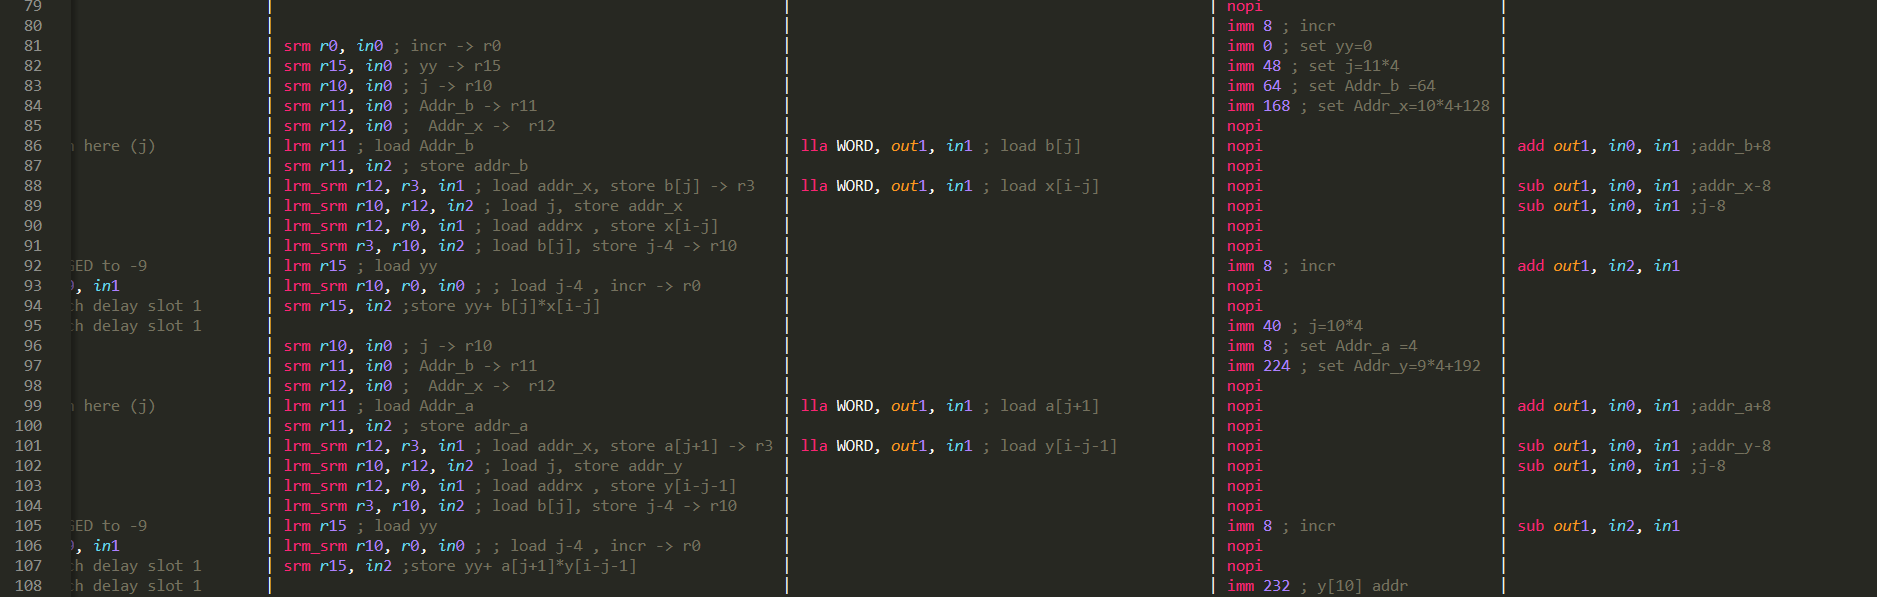
\includegraphics[scale=0.265]{images/assem02.png}
\caption{Excerpt from the Butterworth Filter code from alteration \ref{imp:B}: Loop Halving. Only lines 79 through 108 are shown to clarify alterations to the \texttt{IMM}, \texttt{LSU}, and \texttt{ALU}.}
\label{fig:assem02}
\end{center}
\end{figure}

\subsection{Automatic Addressing}
\label{imp:C}

The exploration of targeting the implicit loading operations lead to negligible improvements. This was expected, as the changes to the code are outside of the main loop, and act as a preemptive optimization. This is completed by changing the \texttt{SLA} operation to a \texttt{SLI} operation with a stride of four. This removes the necessity to compute the memory addresses in the \texttt{ALU} which saves a whopping $42$ cycles.

\begin{figure}[h]
\begin{center}
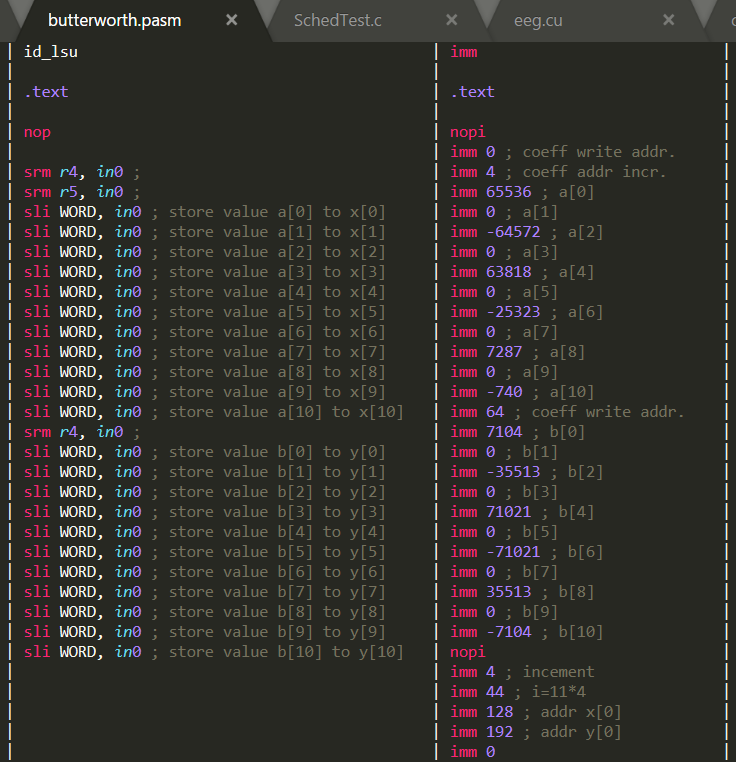
\includegraphics[scale=0.35]{images/assem01.png}
\caption{Excerpt from the Butterworth Filter code from alteration \ref{imp:C}: Automatic Addressing. Only lines 1 through 36 are shown to clarify alterations to the \texttt{IMM} and \texttt{LSU}.}
\label{fig:assem01}
\end{center}
\end{figure}

\subsection{Loop Unpacking}
\label{imp:D}

An attempt was made for loop unpacking, as a colleague informed us they were able to obtain more than $50\%$ improvement over the Naive Butterworth filter. However, this was not realizable due to some undiscoverable errors in the \texttt{PASM} file. The intention was to target the shifting loop \texttt{(x[i-1]=x[i])} and adding an \texttt{LSU} to \texttt{LSU} bypass. The expected results would have been a reduction of $50\%$ or more, and several thousands of cycles in time. Due to time constraints, this implementation will be considered as future work.  

\subsection{Final Architecture}
\label{imp:E}

The resulting architecture is shown below:

\begin{figure}[h]
\begin{center}
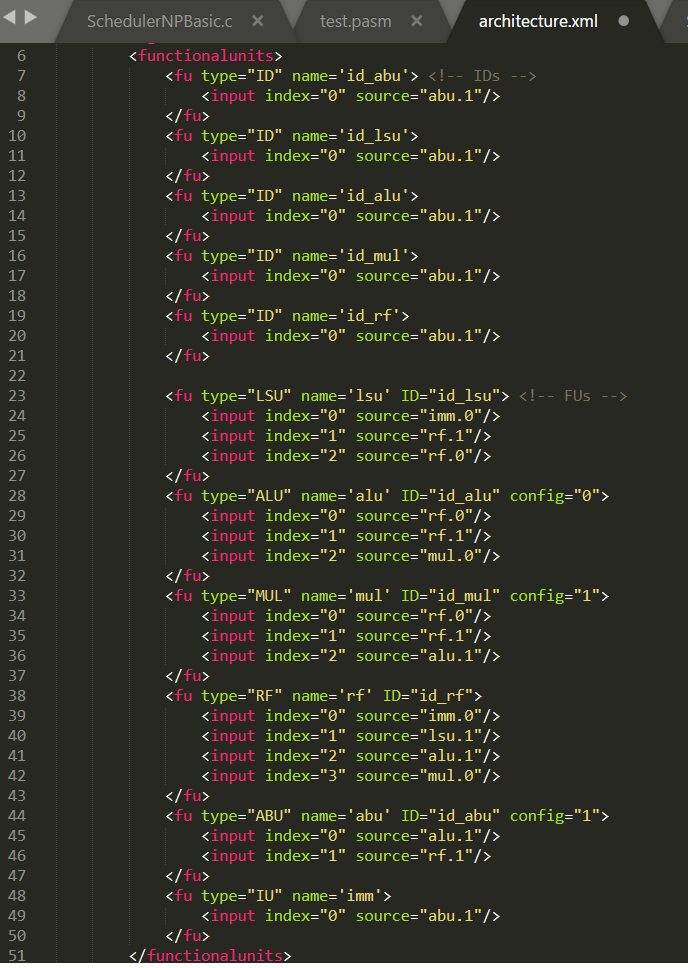
\includegraphics[scale=0.35]{images/arch01.png}
\caption{XML file showing additional connections}
\label{fig:TODO1}
\end{center}
\end{figure}

\begin{figure}[h]
\begin{center}
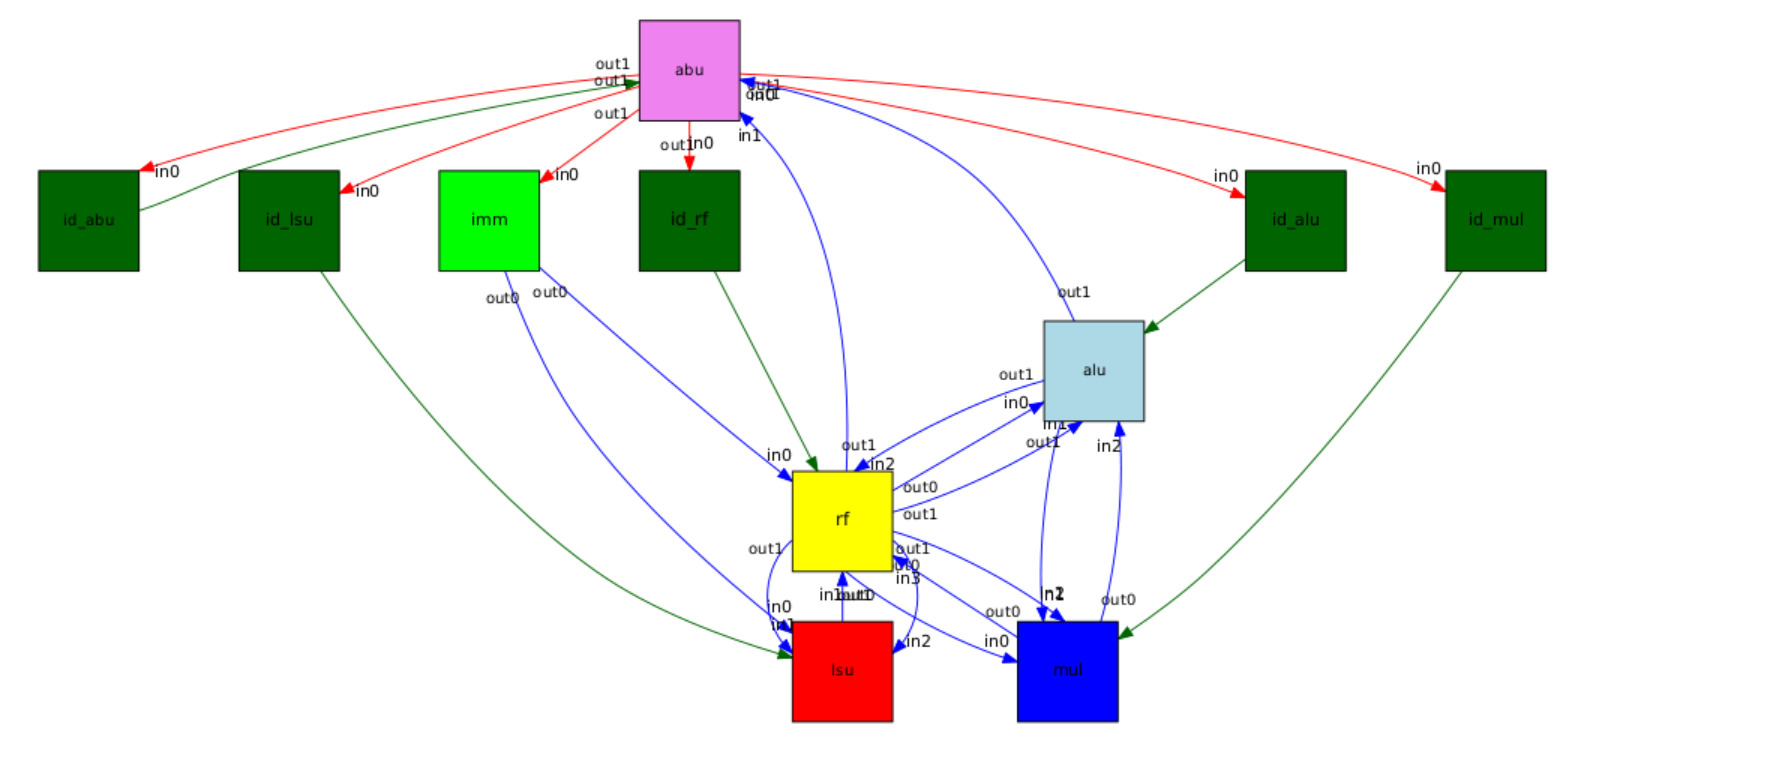
\includegraphics[scale=0.28]{images/arch.png}
\caption{Graphical representation using Xdot Architecture file of new connections.}
\label{fig:TODO2}
\end{center}
\end{figure}


\section{Results}

\begin{table}[h!]
\centering
\caption{Table comparing Duration to Start and End times.}
\label{tab:compare}
\vspace{5pt}
\centering
\begin{tabular}{|l|c|c|c|c|}
\rowcolor[HTML]{C0C0C0}
\hline
 & Naive & Bypass & $\sfrac{1}{2}$ Loop & Auto. Addr. \\ \hline
Energy [pJ] & $8813057.25$  & $8506457.25$ & $6213457.25$ & $6213089.50$ \\ \hline
Cycles & $896146$ & $854146$ & $654146$ & $654104$ \\ \hline
Area [$\mu m^2$] & $89819$ & $90019$ & $90019$ & $90019$ \\ \hline
EDAP & $0.70937$ & $0.65406$ & $0.36588$ & $0.36584$ \\ \hline
$\Delta\pm\%$ (Naive) & $+0.00\%$ & $+7.80\%$ & $+48.42\%$ & $+48.43\%$ \\ \hline

\end{tabular}
\end{table}

\section{Conclusion}

Optimizations were chosen based on suggestions in the supplied cookbook and cooperation in classmates (including the implemented loop-halving and the attempted loop-unpacking). Changing the architecture, algorithms and even C-code reiterates that there are several ways to improve and optimize \texttt{CGRA} performance. Though, given the novelty of the project due to the nature of the \texttt{CGRA}, Toolchain, and \texttt{PASM} setup, it is not easy to debug errors and each iteration must be done with extreme care. As experienced in the loop unpacking attempt, one small error in the \texttt{PASM} may result in uncompilable code (which results in the server timing out after half a million cycles or automatically assuming values for inputs/outputs that are not properly connected).



\begin{figure}[h]
\begin{center}
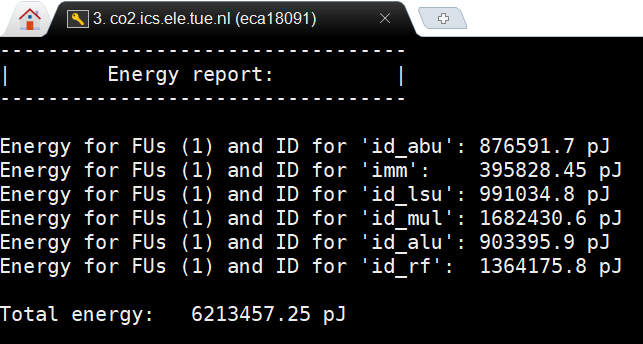
\includegraphics[scale=0.35]{images/O101.png}
\caption{TODO}
\label{fig:TODO3}
\end{center}
\end{figure}

\begin{figure}[h]
\begin{center}
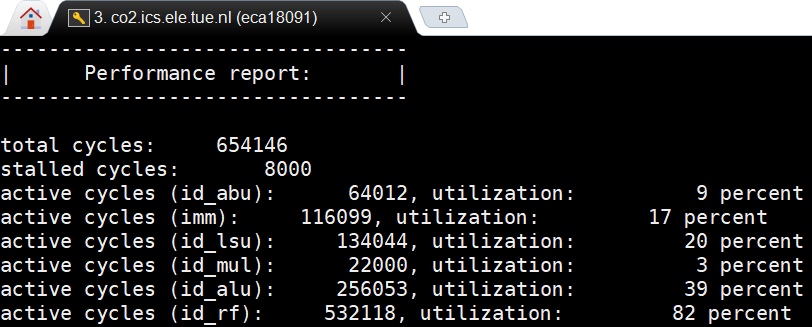
\includegraphics[scale=0.35]{images/O102.png}
\caption{TODO}
\label{fig:TODO4}
\end{center}
\end{figure}

\begin{figure}[h]
\begin{center}
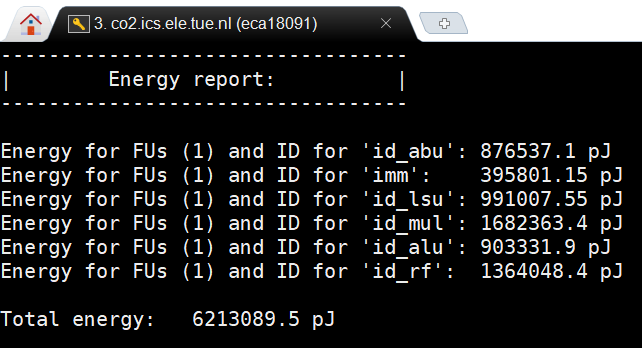
\includegraphics[scale=0.35]{images/O201.png}
\caption{TODO}
\label{fig:TODO5}
\end{center}
\end{figure}

\begin{figure}[h]
\begin{center}
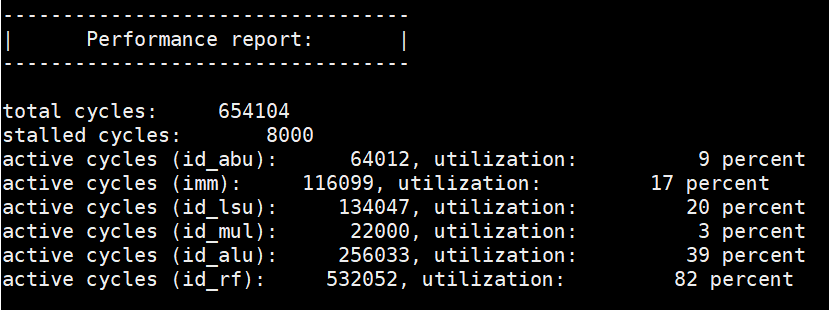
\includegraphics[scale=0.35]{images/O202.png}
\caption{TODO}
\label{fig:TODO6}
\end{center}
\end{figure}













\section{Notes}
Always \texttt{make clean} when changing the files that are being compiled (file name, included files, etc.), to avoid run-time errors, fragmentation errors and output mismatches.

\addtolength{\textheight}{-12cm}   % This command serves to balance the column lengths
                                  % on the last page of the document manually. It shortens
                                  % the textheight of the last page by a suitable amount.
                                  % This command does not take effect until the next page
                                  % so it should come on the page before the last. Make
                                  % sure that you do not shorten the textheight too much.

%%%%%%%%%%%%%%%%%%%%%%%%%%%%%%%%%%%%%%%%%%%%%%%%%%%%%%%%%%%%%%%%%%%%%%%%%%%%%%%%



%%%%%%%%%%%%%%%%%%%%%%%%%%%%%%%%%%%%%%%%%%%%%%%%%%%%%%%%%%%%%%%%%%%%%%%%%%%%%%%%



%%%%%%%%%%%%%%%%%%%%%%%%%%%%%%%%%%%%%%%%%%%%%%%%%%%%%%%%%%%%%%%%%%%%%%%%%%%%%%%%
%\section*{APPENDIX}
%
%Appendixes should appear before the acknowledgment.
%
%\section*{ACKNOWLEDGMENT}
%
%The preferred spelling of the word ÒacknowledgmentÓ in America is without an ÒeÓ after the ÒgÓ. Avoid the stilted expression, ÒOne of us (R. B. G.) thanks . . .Ó  Instead, try ÒR. B. G. thanksÓ. Put sponsor acknowledgments in the unnumbered footnote on the first page.



%%%%%%%%%%%%%%%%%%%%%%%%%%%%%%%%%%%%%%%%%%%%%%%%%%%%%%%%%%%%%%%%%%%%%%%%%%%%%%%%




\begin{thebibliography}{99}

\bibitem{Podder} Prajoy Podder, Md. Mehedi Hasan, Md.Rafiqul Islam, Mursalin Sayeed, Design and Implementation of Butterworth, Chebyshev-I, International Journal of Computer Applications (0975 – 8887), Volume 98– No.7, July 2014.

\bibitem{Neumann} Enticknap, Nicholas. (1989). VON NEUMANN ARCHITECTURE. 128-129. 10.1016/B978-1-4831-3553-3.50066-9. 




\end{thebibliography}




\end{document}
